\begin{figure*}
\begin{minipage}{0.55\linewidth}
  \centerline{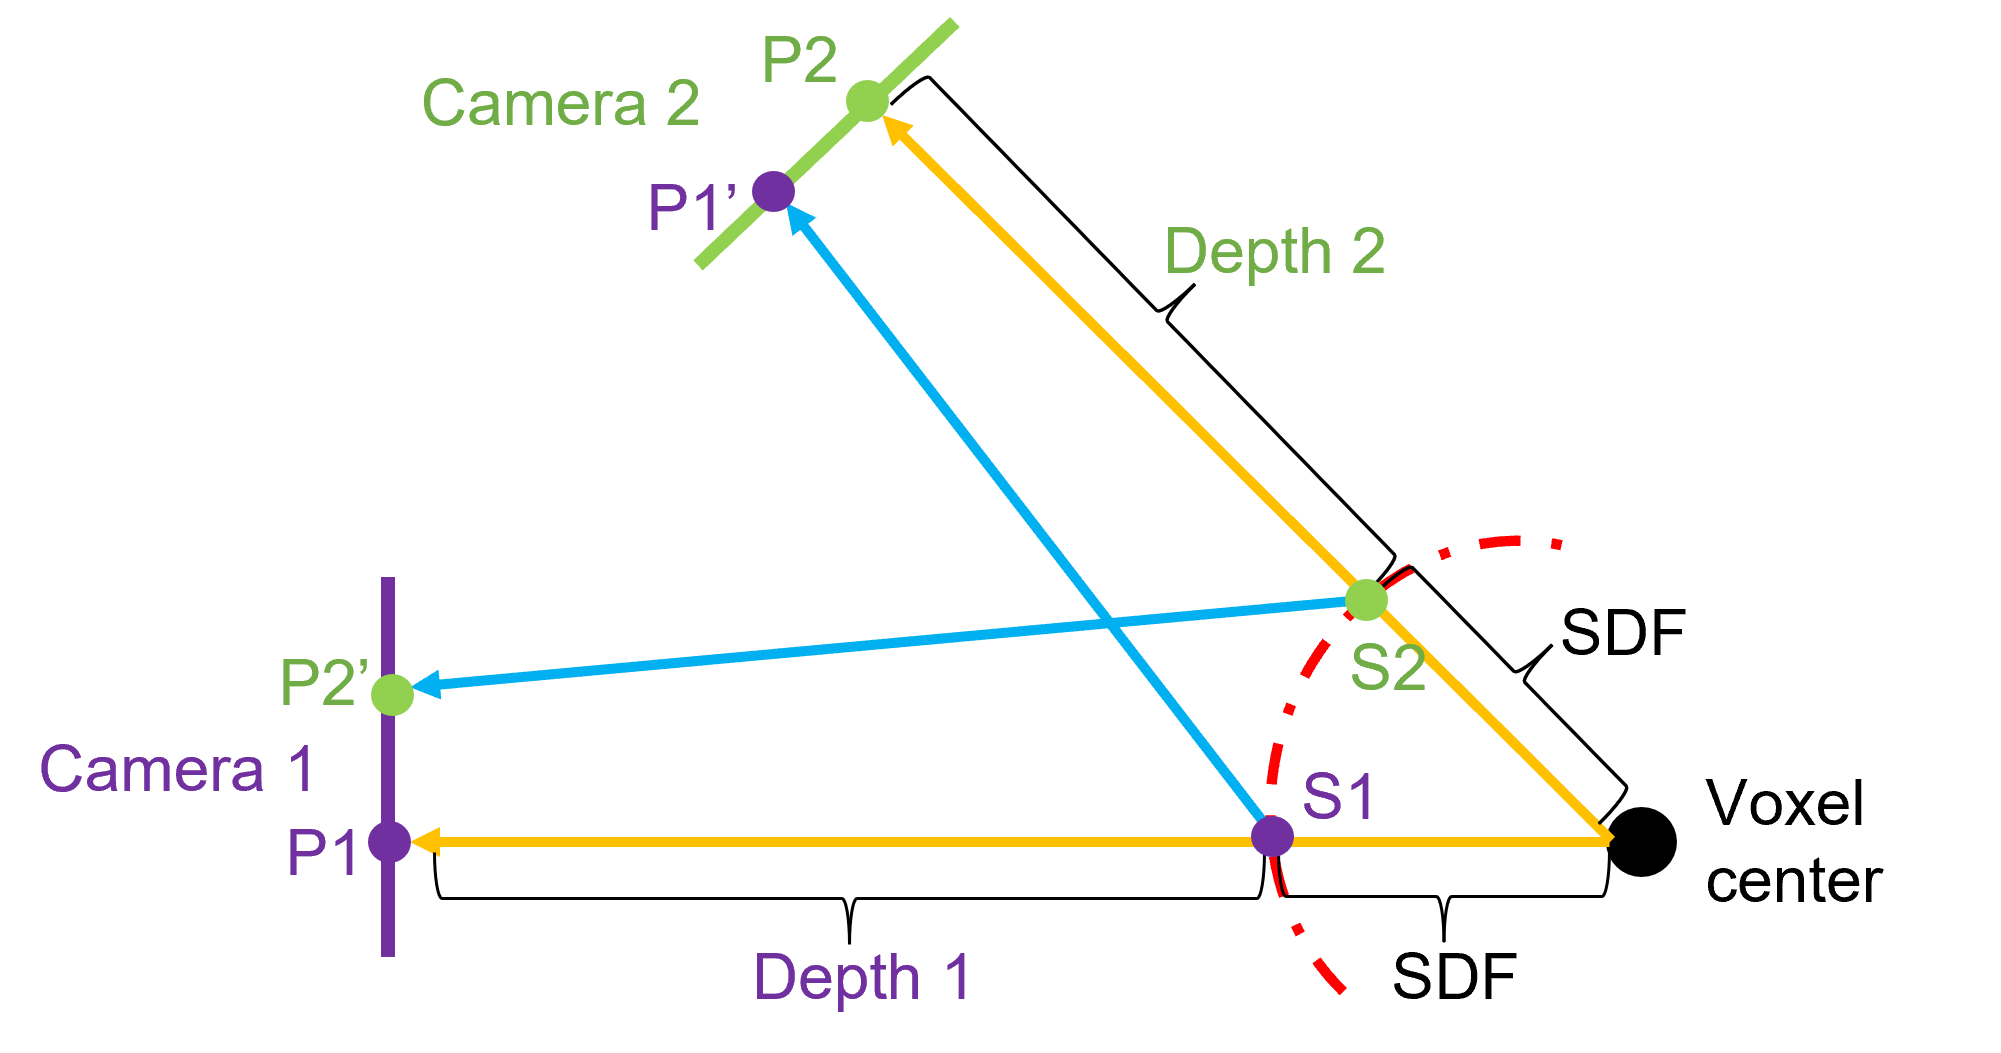
\includegraphics[width=1.0\textwidth]{figures/sdf_loss_a.png}}
\end{minipage}
\hfill
\begin{minipage}{0.51\linewidth}
  \centerline{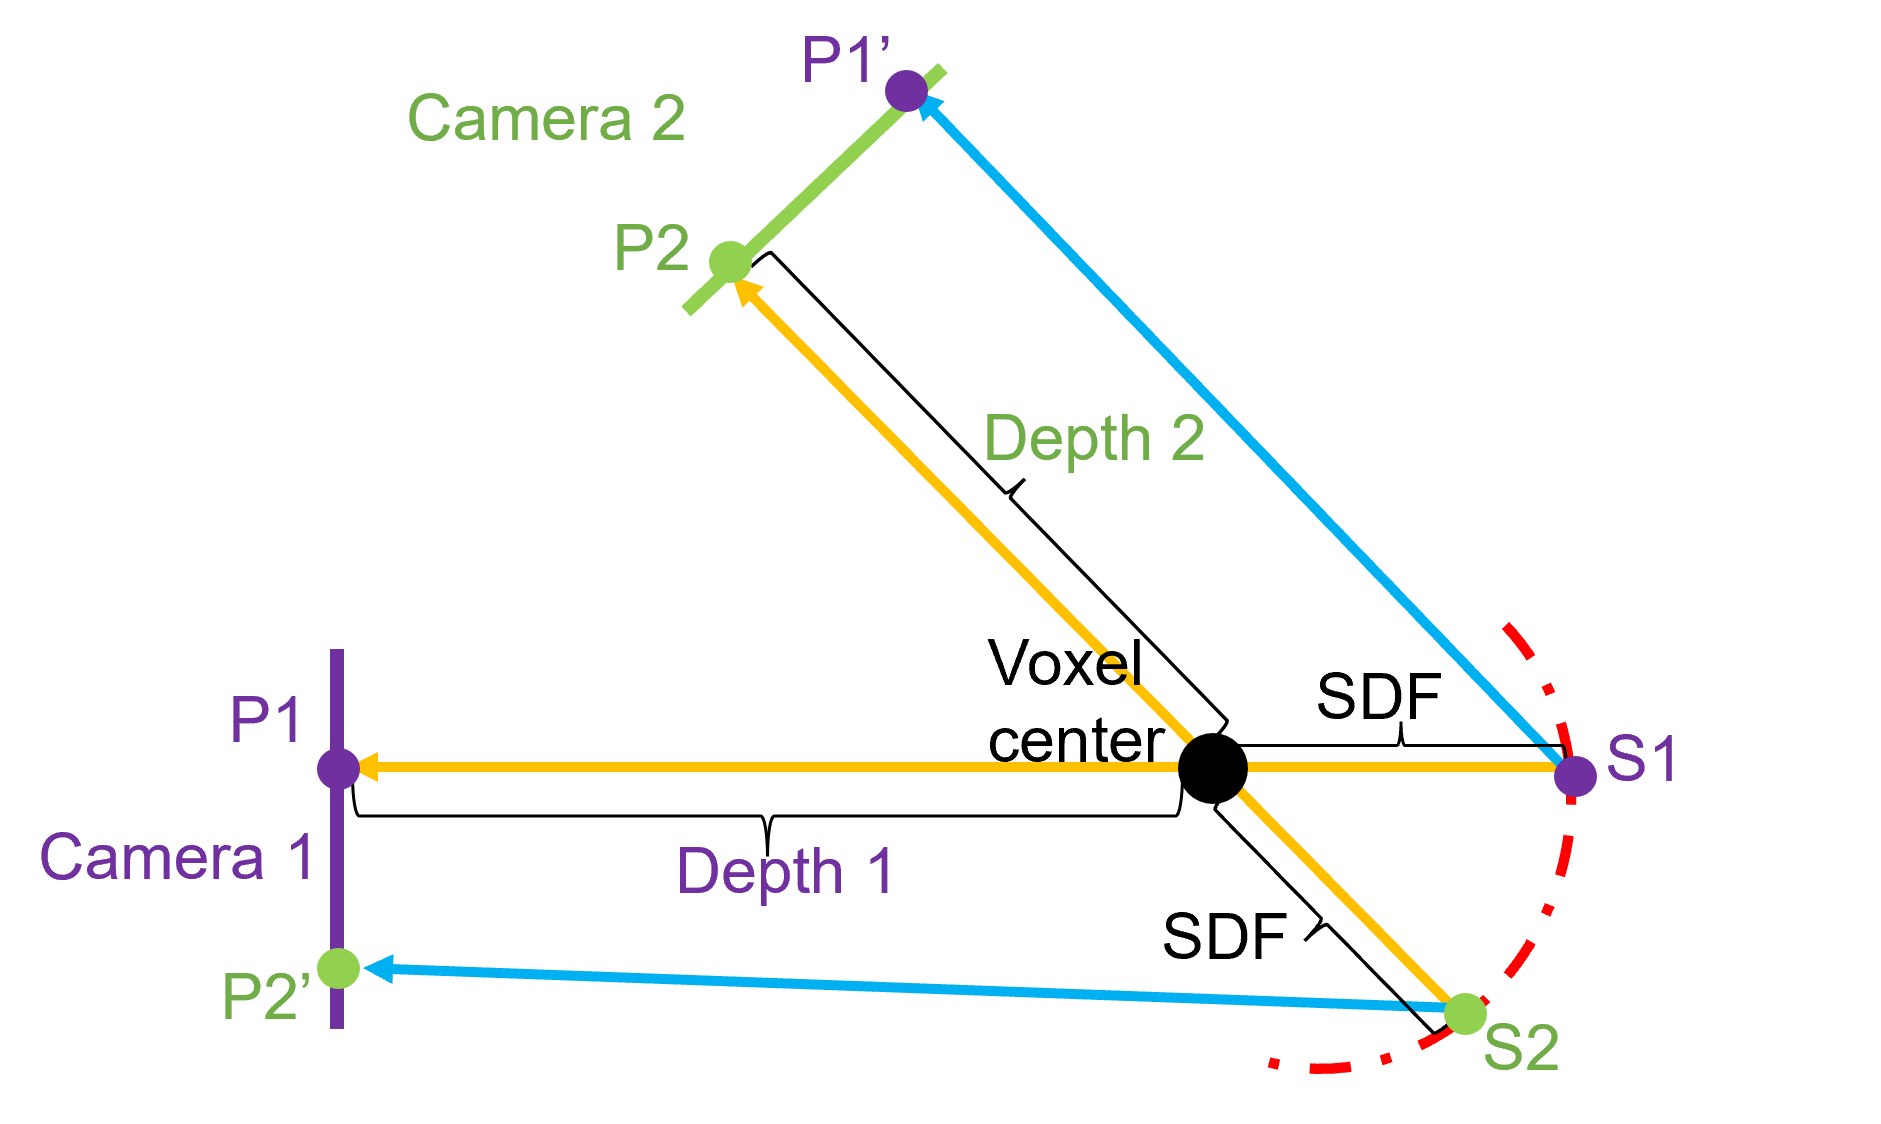
\includegraphics[width=1.0\textwidth]{figures/sdf_loss_b.png}}
\end{minipage}
\vspace{-5mm}
\caption{\textbf{Self-supervised SDF photometric loss between source and target views}. \textbf{Left:} Voxel center is inside of the surface, SDF is negative. Orange arrows show projecting rays from voxel centers to 2D pixels (P1, P2) on each camera plane, blue arrows show reprojection of surface 3D points (S1, S2) to 2D pixels (P1', P2') in each camera plane. Surface points are estimated by SDF estimation. \textbf{Right:} Voxel center is outside of the surface, SDF is positive. \textbf{The loss is extended to all n views in a fragment}.}
\label{fig:sdf photometric loss}
\vspace{-5mm}
\end{figure*}

\vspace{-2mm}
\section{Method}
\label{sec:method}
\vspace{-2mm}
\subsection{MonoSelfRecon Framework}
\quad Figure \ref{fig:pipeline} shows our MonoSelfRecon framework. In both training and testing, we take the input monocular RGB sequence and camera poses, and reconstruct 3D mesh of the whole scene. We select key frames following the process in \cite{key_select}, where we consider a valid frame to be ``greater than 15 degree in rotation or 0.3 meter in translation'' to the previous frame. Every $n$ consecutive key frames form a scene fragment. Fragments are fed as inputs, from which, the network extracts 2D features per key frame, creates 3D feature volume and jointly estimates SDF and NeRF using separate decoders at three pyramid scales. In SDF decoder, 2D features are fused to 3D voxel features and regress to voxel-SDF values at each level with 3D sparse convolution. Every time the network only estimates SDF corresponding to the fragment in a $[N,N,N]$ 3D voxel region, the Gated Recurrent Unit (GRU) module at each level updates SDF, fuses reconstruction from previous fragments, and completes the whole scene. During training, self-supervised losses are implemented between SDF-input, NeRF-input, and SDF-NeRF, with detailed discussion in \ref{sec:losses}. During testing, 3D mesh can be obtained from SDF through marching cube\cite{marchingcube}.  

\noindent
\textbf{Attentional View Fusion}.
For each fragment, 3D voxel features can be simply obtained by projecting the 3D voxel to each 2D view in the fragment, searching for visible corresponding pixels, and averaging 2D features. However, since each view have different distance, angle, and occlusion to voxels, 2D features from different views should not contribute the same to 3D features. Inspired by recent works \cite{vortx}, we use an attentional view fusion module by adding a light transformer before averaging features. The transformer takes unordered sequence of 2D features and updates weighted features before average to 3D, which enables more flexibility to adjust the contribution of each frame to the fragment. Although simple, this module achieves significant improvement as shown in the ablation study in Table \ref{table:scannet_ablation}.

\noindent
\textbf{GRU}. 
We adapt the GRU module from \cite{neucon}. With camera poses, it is simple to concatenate fragments and replace the overlapping voxels of latter fragment to the previous one, but it ignores the effect of the latter views to the previous ones. Once fusing 3D voxel features from 2D and before regressing voxel-SDF at each level, the GRU module takes 3D voxel features of both previous and current fragments as input to update the current features. GRU fusion makes an obvious improvement as shown in the ablation study in Table \ref{table:scannet_ablation}. 


\noindent
\textbf{NeRF.} We adopt the generalizable MPI (MultiPlane-Images)-NeRF \cite{mpi, mpi-nerf, mononerf}, introduce it to the framework and jointly train with SDF to boost SDF estimation. The core idea is to use an explicit encoder on top of standard positional encoding to enable implicit NeRF with generalization ability. The NeRF estimation also further boosts our SDF performance as shown in the ablation study in Table \ref{table:scannet_ablation}.

\subsection{Self-supervised Losses}
\label{sec:losses}

\noindent
\textbf{SDF Photometric Loss}. Figure \ref{fig:sdf photometric loss} shows a simplified version of the loss implementation between two camera views, where the corresponding 2D coordinates (P1 and P2) can be found by tracing rays (orange arrows) to camera planes. SDF is the distance between a point to its nearest surface, where the value is negative when the point is inside of the surface, and positive when it is outside of the surface. The model estimates SDF per voxel. The depth $\hat{D}_{cam}$ can be estimated by Eq. \ref{eq:get_depth}, where $V_{world}$ is 3D world coordinate of the pre-defined voxel center, $T_{world\xrightarrow{}cam}$ is camera extrinsic, $\hat{SDF}$ is the estimated voxel-SDF from the model. With depth and voxel center in the camera coordinate, the surface points S1 and S2 can be estimated by Eq. \ref{eq:get_surface}, where $\vec{ray}$ is the unit vector at ray direction (orange arrows), and $\hat{S}_{cam}$ is the 3D coordinate of a surface point in the camera view. Finally, the reconstructed pixels are obtained by reprojecting (blue arrows) surface points S1, S2 to camera 2 and 1 as Eq. \ref{eq:point_proj}, where K is camera intrinsic, $T_{cam\xrightarrow{}cam'}$ is camera pose from cam to cam'. P-P' is a pixel reconstruction pair with same photometric intensity, where a photometric consistency loss can be derived as Eq. \ref{eq:pts_loss}. The exact pixel intensities $I_{cam}(P)$ and $I_{cam'}(P')$ are obtained with bilinear interpolation from projected 2D points lying between integer coordinates, and the loss is only traced to the points lying within the camera planes.
\vspace{-3mm}
\begin{equation}
\begin{split}
    V_{cam} = T_{world\xrightarrow{}cam}V_{world} \\
    \hat{D}_{cam} = V_{cam} + \hat{SDF}
    \label{eq:get_depth}
\end{split}
\end{equation}
\vspace{-6mm}

\vspace{-5mm}
\begin{equation}
\begin{split}
    \hat{S}_{cam}(x, y, z) = V_{cam}(x, y, z) + |\hat{SDF}| \Vec{ray}(x, y, z)
    \label{eq:get_surface}
\end{split}
\end{equation}
\vspace{-6mm}

\vspace{-5mm}
\begin{equation}
\begin{split}
    P = Interp(KV_{cam}) \\
    P' = Interp(K'T_{cam\xrightarrow{}cam'}\hat{S}_{cam})
\end{split}
\label{eq:point_proj}
\end{equation}
\vspace{-6mm}

\vspace{-4mm}
\begin{equation}
    L_{sdf} = \sum_{P \in cam}\sum_{P'\in cam'}{|(I_{cam}(P) - I_{cam'}(P')|}
\label{eq:pts_loss}
\end{equation}
\vspace{-4mm}

\iffalse
We make an assumption to set up this point-wise self-supervised SDF loss. Although the distance from the voxel center to different surface points varies - only the nearest distance is SDF. Since the network estimates one SDF value per voxel, we use the same estimated SDF value corresponding to the same voxel center to estimate surface points for different camera views. However, previous supervised works made the same assumption to implement TSDF fusion  \cite{atlas, neucon} and get TSDF ground truth from the depth map. More specifically, instead of using the nearest distance, they take the average distances from all views. Similarly, we assign this task to the network, when the resolution is large enough (voxel size is small enough), the network is trained to get to the average distance that optimizes the consistency loss between all camera views.
\fi

In practice, we implement the loss across all views in the scene fragment and take the weighted average loss, where the weight is in direct proportion to the number of the candidate P-P' pair. If P' lies outside of the other camera's plane, we ignore this P-P' pair. For SFM-based self-supervised depth works, they start from 2D pixel and ends up at 2D pixel to jointly regress depth and camera pose. However, we start from 3D voxel center and end up at 2D pixel to only regress the depth model while taking camera pose as prior, which is why SFM-based self-supervised depth estimation has scale ambiguity, while our SDF estimation is directly in real scale. 

\noindent
\textbf{SDF Co-Planar Loss}. Photometric constraints are insufficient for indoors scenes due to large non-textured regions and in-plane rotations. Thus, we take advantage of the special geometric constraints in indoor scenes. Most indoor scenes have large planes such as walls, floors, and ceilings, where textures within such planes are mostly similar. Inspired by \cite{p2net, planercnn, planenet, piece-wise} that implement planar constraints in 2D depth maps, we extend it to 3D SDF. Specifically, we adopted `Felzenszwalb superpixel segmentation' \cite{plane_seg} to extract `super-pixels', which covers piece-wise large group of regions that have low pixel intensity gradients, which are considered as a planar region. The algorithm uses greedy search to extract super-pixels and is free of learning. Based on the planar segmentation and the depth planar constraints from \cite{structdepth}, we propose a voxel-SDF driven co-planar loss.

Our goal is to derive plane parameters under planar constraints, and learn the plane parameters in a self-supervised manner. Specifically, the plane segmentation extracts $n$ super-pixels from a 2D image, with each super-pixel corresponding to a continuous plane. For the 2D projected voxel center point P (as shown in Figure \ref{fig:sdf photometric loss}), if it belongs to super-pixel $SP_m$ in the 2D plane, then the surface 3D point $S$ corresponding to $P$ also belongs to the surface plane of class $m$ in 3D space. Using the surface point $S$, the plane $m$ can be defined as Eq. \ref{eq:plane_onepoint}, where $\hat{s}_{0}$ is an estimated surface point in the plane, and $A_m$ is the plane parameter.

\vspace{-3mm}
\begin{equation}
    A_{m}^T \hat{s}_{0} = 1
    \label{eq:plane_onepoint}
\end{equation}
\vspace{-5mm}

While using only one 3D point to simulate a plane is ill-posed, a large number of estimated 3D surface points are obtained by projecting voxel centers to different camera views. With $n$ 2D projected points $p_1$, $p_2$ ...... $p_n$ belonging to super-pixel $SP_m$, there are $n$ 3D surface points $s_1$, $s_2$, ......, $s_n$ belonging to 3D surface plane $m$. Eq. \ref{eq:plane_onepoint} is extended to Eq. \ref{eq:plane_npoint}, where $\hat{S}_{n} = [\hat{s}_{1}, \hat{s}_{2}, ......, \hat{s}_{n}]$, and $Y_m = \Vec{1} = [1,1,...,1]$.

\vspace{-3mm}
\begin{equation}
    \hat{S}_{n} A_{m}^T  = Y_{m}
    \label{eq:plane_npoint}
\end{equation}
\vspace{-5mm}

The plane parameter $A_{m}$ is then estimated by least-square method as Eq. \ref{eq:least_square}, where $\epsilon$ is a small scalar for stability, and $I$ is an identity matrix.

\vspace{-3mm}
\begin{equation}
    A_m = (\hat{S}_n^T\hat{S}_n+\epsilon I)^{-1}\hat{S}_n^TY_m
    \label{eq:least_square}
\end{equation}
\vspace{-5mm}

With the estimated plane parameter, the pseudo surface points can be retrieve  by $\hat{S_n}' = (A_m^T \hat{S_n})^{-1}$. The pseudo surface and estimated surface are expected to align together, and we implement such a co-planar geometric constraint as the self-supervised co-planar SDF loss as Eq. \ref{eq:plane_loss}.

\vspace{-3mm}
\begin{equation}
    L_{plane} = \sum_{M}\sum_{N}{|\hat{S_n}-\hat{S_n}'|}
\label{eq:plane_loss}
\end{equation}
\vspace{-3mm}

\noindent
\textbf{Depth Consistency Loss.} We also propose depth consistency loss to further boost SDF from NeRF. Specifically, we estimate sparse Pseudo-SDF depth for target views from estimated SDF (as Figure \ref{fig:sdf photometric loss}), and render NeRF-depth for corresponding target views. Since Pseudo-SDF depth is in real scale, we first use it to recover NeRF-depth's scale, and enforce consistency between the two estimated depths. 

\vspace{-3mm}
\begin{equation}
    L_{depth} = \sum_{N}\sum_{D \in cam}{|\hat{D_{sdf}}-\hat{D_{NeRF}}|}
\label{eq:depth_loss}
\end{equation}
\vspace{-3mm}

\noindent
where $\hat{D_{sdf}}$ and $\hat{D_{NeRF}}$ are Pseudo-SDF depth and the scale-recoverd NeRF-depth, respectively.

\noindent
\textbf{Total Loss.} We implement standard NeRF losses for NeRF encoder, including RGB consistency with input images, SSIM, and smooth loss, and we jointly train everything end-to-end in pure self-supervision.

\vspace{-8mm}
\begin{equation}
    L_{NeRF} = L_{rgb} + L_{smooth} + (1 - SSIM)
\label{eq:nerf_loss}
\end{equation}
\vspace{-6mm}

\noindent
The total loss is the weighted sum of all losses, where $\lambda$s are the weights,

\vspace{-3mm}
\begin{multline}
    L_{total} = \lambda_{sdf}L_{sdf} + \lambda_{plane}L_{plane} \\ + 
    \lambda_{depth}L_{depth} + \lambda_{NeRF}L_{NeRF}
\label{eq:total_loss}
\end{multline}
\vspace{-5mm}